% Options for packages loaded elsewhere
\PassOptionsToPackage{unicode}{hyperref}
\PassOptionsToPackage{hyphens}{url}
\PassOptionsToPackage{dvipsnames,svgnames*,x11names*}{xcolor}
%
\documentclass[
  10pt,
  dvipsnames,enabledeprecatedfontcommands]{scrartcl}
\usepackage{amsmath,amssymb}
\usepackage{lmodern}
\usepackage{ifxetex,ifluatex}
\ifnum 0\ifxetex 1\fi\ifluatex 1\fi=0 % if pdftex
  \usepackage[T1]{fontenc}
  \usepackage[utf8]{inputenc}
  \usepackage{textcomp} % provide euro and other symbols
\else % if luatex or xetex
  \usepackage{unicode-math}
  \defaultfontfeatures{Scale=MatchLowercase}
  \defaultfontfeatures[\rmfamily]{Ligatures=TeX,Scale=1}
\fi
% Use upquote if available, for straight quotes in verbatim environments
\IfFileExists{upquote.sty}{\usepackage{upquote}}{}
\IfFileExists{microtype.sty}{% use microtype if available
  \usepackage[]{microtype}
  \UseMicrotypeSet[protrusion]{basicmath} % disable protrusion for tt fonts
}{}
\makeatletter
\@ifundefined{KOMAClassName}{% if non-KOMA class
  \IfFileExists{parskip.sty}{%
    \usepackage{parskip}
  }{% else
    \setlength{\parindent}{0pt}
    \setlength{\parskip}{6pt plus 2pt minus 1pt}}
}{% if KOMA class
  \KOMAoptions{parskip=half}}
\makeatother
\usepackage{xcolor}
\IfFileExists{xurl.sty}{\usepackage{xurl}}{} % add URL line breaks if available
\IfFileExists{bookmark.sty}{\usepackage{bookmark}}{\usepackage{hyperref}}
\hypersetup{
  pdftitle={Taking uncertainty in word embedding bias estimation seriously: a bayesian approach},
  pdfauthor={Alicja Dobrzeniecka and Rafal Urbaniak},
  colorlinks=true,
  linkcolor=Maroon,
  filecolor=Maroon,
  citecolor=Blue,
  urlcolor=blue,
  pdfcreator={LaTeX via pandoc}}
\urlstyle{same} % disable monospaced font for URLs
\usepackage{color}
\usepackage{fancyvrb}
\newcommand{\VerbBar}{|}
\newcommand{\VERB}{\Verb[commandchars=\\\{\}]}
\DefineVerbatimEnvironment{Highlighting}{Verbatim}{commandchars=\\\{\}}
% Add ',fontsize=\small' for more characters per line
\usepackage{framed}
\definecolor{shadecolor}{RGB}{248,248,248}
\newenvironment{Shaded}{\begin{snugshade}}{\end{snugshade}}
\newcommand{\AlertTok}[1]{\textcolor[rgb]{0.94,0.16,0.16}{#1}}
\newcommand{\AnnotationTok}[1]{\textcolor[rgb]{0.56,0.35,0.01}{\textbf{\textit{#1}}}}
\newcommand{\AttributeTok}[1]{\textcolor[rgb]{0.77,0.63,0.00}{#1}}
\newcommand{\BaseNTok}[1]{\textcolor[rgb]{0.00,0.00,0.81}{#1}}
\newcommand{\BuiltInTok}[1]{#1}
\newcommand{\CharTok}[1]{\textcolor[rgb]{0.31,0.60,0.02}{#1}}
\newcommand{\CommentTok}[1]{\textcolor[rgb]{0.56,0.35,0.01}{\textit{#1}}}
\newcommand{\CommentVarTok}[1]{\textcolor[rgb]{0.56,0.35,0.01}{\textbf{\textit{#1}}}}
\newcommand{\ConstantTok}[1]{\textcolor[rgb]{0.00,0.00,0.00}{#1}}
\newcommand{\ControlFlowTok}[1]{\textcolor[rgb]{0.13,0.29,0.53}{\textbf{#1}}}
\newcommand{\DataTypeTok}[1]{\textcolor[rgb]{0.13,0.29,0.53}{#1}}
\newcommand{\DecValTok}[1]{\textcolor[rgb]{0.00,0.00,0.81}{#1}}
\newcommand{\DocumentationTok}[1]{\textcolor[rgb]{0.56,0.35,0.01}{\textbf{\textit{#1}}}}
\newcommand{\ErrorTok}[1]{\textcolor[rgb]{0.64,0.00,0.00}{\textbf{#1}}}
\newcommand{\ExtensionTok}[1]{#1}
\newcommand{\FloatTok}[1]{\textcolor[rgb]{0.00,0.00,0.81}{#1}}
\newcommand{\FunctionTok}[1]{\textcolor[rgb]{0.00,0.00,0.00}{#1}}
\newcommand{\ImportTok}[1]{#1}
\newcommand{\InformationTok}[1]{\textcolor[rgb]{0.56,0.35,0.01}{\textbf{\textit{#1}}}}
\newcommand{\KeywordTok}[1]{\textcolor[rgb]{0.13,0.29,0.53}{\textbf{#1}}}
\newcommand{\NormalTok}[1]{#1}
\newcommand{\OperatorTok}[1]{\textcolor[rgb]{0.81,0.36,0.00}{\textbf{#1}}}
\newcommand{\OtherTok}[1]{\textcolor[rgb]{0.56,0.35,0.01}{#1}}
\newcommand{\PreprocessorTok}[1]{\textcolor[rgb]{0.56,0.35,0.01}{\textit{#1}}}
\newcommand{\RegionMarkerTok}[1]{#1}
\newcommand{\SpecialCharTok}[1]{\textcolor[rgb]{0.00,0.00,0.00}{#1}}
\newcommand{\SpecialStringTok}[1]{\textcolor[rgb]{0.31,0.60,0.02}{#1}}
\newcommand{\StringTok}[1]{\textcolor[rgb]{0.31,0.60,0.02}{#1}}
\newcommand{\VariableTok}[1]{\textcolor[rgb]{0.00,0.00,0.00}{#1}}
\newcommand{\VerbatimStringTok}[1]{\textcolor[rgb]{0.31,0.60,0.02}{#1}}
\newcommand{\WarningTok}[1]{\textcolor[rgb]{0.56,0.35,0.01}{\textbf{\textit{#1}}}}
\usepackage{graphicx}
\makeatletter
\def\maxwidth{\ifdim\Gin@nat@width>\linewidth\linewidth\else\Gin@nat@width\fi}
\def\maxheight{\ifdim\Gin@nat@height>\textheight\textheight\else\Gin@nat@height\fi}
\makeatother
% Scale images if necessary, so that they will not overflow the page
% margins by default, and it is still possible to overwrite the defaults
% using explicit options in \includegraphics[width, height, ...]{}
\setkeys{Gin}{width=\maxwidth,height=\maxheight,keepaspectratio}
% Set default figure placement to htbp
\makeatletter
\def\fps@figure{htbp}
\makeatother
\setlength{\emergencystretch}{3em} % prevent overfull lines
\providecommand{\tightlist}{%
  \setlength{\itemsep}{0pt}\setlength{\parskip}{0pt}}
\setcounter{secnumdepth}{5}
%\documentclass{article}

% %packages
\usepackage{booktabs}
%\usepackage[left]{showlabels}
\usepackage{multirow}
\usepackage{subcaption}

\usepackage{graphicx}
%\usepackage{longtable}
\usepackage{supertabular, booktabs}
\usepackage{ragged2e}
\usepackage{etex}
%\usepackage{yfonts}
\usepackage{marvosym}
\usepackage[notextcomp]{kpfonts}
\usepackage{nicefrac}
\newcommand*{\QED}{\hfill \footnotesize {\sc Q.e.d.}}
\usepackage{floatrow}

\usepackage[textsize=footnotesize]{todonotes}
\newcommand{\ali}[1]{\todo[color=gray!40]{\textbf{Alicja:} #1}}
\newcommand{\mar}[1]{\todo[color=blue!40]{#1}}
\newcommand{\raf}[1]{\todo[color=olive!40]{#1}}

%\linespread{1.5}
\newcommand{\indep}{\!\perp \!\!\! \perp\!}


\setlength{\parindent}{10pt}
\setlength{\parskip}{1pt}


%language
%\usepackage{times}
\usepackage{mathptmx}
\usepackage[scaled=0.86]{helvet}
\usepackage{t1enc}
%\usepackage[utf8x]{inputenc}
%\usepackage[polish]{babel}
%\usepackage{polski}




%AMS
\usepackage{amsfonts}
\usepackage{amssymb}
\usepackage{amsthm}
\usepackage{amsmath}
\usepackage{mathtools}

\usepackage{geometry}
 \geometry{a4paper,left=35mm,top=20mm,}


%environments
\newtheorem{fact}{Fact}



%abbreviations
\newcommand{\ra}{\rangle}
\newcommand{\la}{\langle}
\newcommand{\n}{\neg}
\newcommand{\et}{\wedge}
\newcommand{\jt}{\rightarrow}
\newcommand{\ko}[1]{\forall  #1\,}
\newcommand{\ro}{\leftrightarrow}
\newcommand{\exi}[1]{\exists\, {_{#1}}}
\newcommand{\pr}[1]{\ensuremath{\mathsf{P}(#1)}}
\newcommand{\cost}{\mathsf{cost}}
\newcommand{\benefit}{\mathsf{benefit}}
\newcommand{\ut}{\mathsf{ut}}

\newcommand{\odds}{\mathsf{Odds}}
\newcommand{\ind}{\mathsf{Ind}}
\newcommand{\nf}[2]{\nicefrac{#1\,}{#2}}
\newcommand{\R}[1]{\texttt{#1}}
\newcommand{\prr}[1]{\mbox{$\mathtt{P}_{prior}(#1)$}}
\newcommand{\prp}[1]{\mbox{$\mathtt{P}_{posterior}(#1)$}}



\newtheorem{q}{\color{blue}Question}
\newtheorem{lemma}{Lemma}
\newtheorem{theorem}{Theorem}
\newtheorem{corollary}{Corollary}[fact]


%technical intermezzo
%---------------------

\newcommand{\intermezzoa}{
	\begin{minipage}[c]{13cm}
	\begin{center}\rule{10cm}{0.4pt}



	\tiny{\sc Optional Content Starts}
	
	\vspace{-1mm}
	
	\rule{10cm}{0.4pt}\end{center}
	\end{minipage}\nopagebreak 
	}


\newcommand{\intermezzob}{\nopagebreak 
	\begin{minipage}[c]{13cm}
	\begin{center}\rule{10cm}{0.4pt}

	\tiny{\sc Optional Content Ends}
	
	\vspace{-1mm}
	
	\rule{10cm}{0.4pt}\end{center}
	\end{minipage}
	}
	
	
%--------------------






















\newtheorem*{reply*}{Reply}
\usepackage{enumitem}
\newcommand{\question}[1]{\begin{enumerate}[resume,leftmargin=0cm,labelsep=0cm,align=left]
\item #1
\end{enumerate}}

\usepackage{float}

\usepackage{sectsty}
\sectionfont{\fontsize{11}{11}\selectfont}

% \setbeamertemplate{blocks}[rounded][shadow=true]
% \setbeamertemplate{itemize items}[ball]
% \AtBeginPart{}
% \AtBeginSection{}
% \AtBeginSubsection{}
% \AtBeginSubsubsection{}
% \setlength{\emergencystretch}{0em}
% \setlength{\parskip}{0pt}






\usepackage[authoryear]{natbib}

%\bibliographystyle{apalike}



\usepackage{tikz}
\usetikzlibrary{positioning,shapes,arrows}

\ifluatex
  \usepackage{selnolig}  % disable illegal ligatures
\fi
\newlength{\cslhangindent}
\setlength{\cslhangindent}{1.5em}
\newlength{\csllabelwidth}
\setlength{\csllabelwidth}{3em}
\newenvironment{CSLReferences}[2] % #1 hanging-ident, #2 entry spacing
 {% don't indent paragraphs
  \setlength{\parindent}{0pt}
  % turn on hanging indent if param 1 is 1
  \ifodd #1 \everypar{\setlength{\hangindent}{\cslhangindent}}\ignorespaces\fi
  % set entry spacing
  \ifnum #2 > 0
  \setlength{\parskip}{#2\baselineskip}
  \fi
 }%
 {}
\usepackage{calc}
\newcommand{\CSLBlock}[1]{#1\hfill\break}
\newcommand{\CSLLeftMargin}[1]{\parbox[t]{\csllabelwidth}{#1}}
\newcommand{\CSLRightInline}[1]{\parbox[t]{\linewidth - \csllabelwidth}{#1}\break}
\newcommand{\CSLIndent}[1]{\hspace{\cslhangindent}#1}

\title{Taking uncertainty in word embedding bias estimation seriously: a
bayesian approach}
\author{Alicja Dobrzeniecka and Rafal Urbaniak}
\date{}

\begin{document}
\maketitle

\hypertarget{cosine-based-measures-of-bias}{%
\section{Cosine-based measures of
bias}\label{cosine-based-measures-of-bias}}

\hypertarget{word-embeddings-and-their-bias}{%
\subsection{Word embeddings and their
bias}\label{word-embeddings-and-their-bias}}

Modern Natural Language Processing (NLP) models are used to complete
various tasks such as providing email filters, smart assistants, search
results, language translations, text analytics and so on. All of them
need as an input words represented by means of numbers which is
accomplished with word embeddings, in which particular lexical units are
represented as vectors of real numbers. They are necessary to perform
machine learning tasks that require the use of natural language. One of
the ways to learn these vectors representations is to use simple neural
network that based on the millions of real sentences examples assigns
the numbers based on their co-occurrence and context. Using co-occurence
results in a vector space that contains similar words closer to each
other and dissimilar further away. It has been suggested {[}1--6{]} that
in the learning process such models can learn implicit biases that
reflect harmful stereotypical thinking (eg. that the word \textit{she}
is much closer in the vector space to the word \textit{cooking} than the
word \textit{he}). This phenomenon may be undesired when using these
vectors for further downstream tasks (eg. web search, recommendations,
etc.).\todo{find downstream tasks and bias examples from papers} Before
we move to more technical details regarding this topic, it is worth
looking first at the theoretical background which may help to better
grasp the concept of bias within machine learning algorithms.

In \todo{cite Are algorithms Value-Free} the author focuses on the
general issue, namely whether algorithms can in principle be value-free.
The author draws attention to the observation that in both scientific
research and machine learning domain, induction plays a crucial role in
the decision-making process. Induction is essential for both of these
domains as ``if ever considered literally just the facts, we would never
be able to draw inductive conclusions'' \todo{cite Gabrielle}. Induction
comes with certain risks which are 1) the problem with justification,
and 2) the risk of getting things wrong. During the process of designing
machine learning process some decisions have to always be made. As the
author states, there is no such thing as the justification in the
abstract. \todo{cite Gabrielle} We may justify certain design decisions,
data choice, etc. only by referring to the world's being certain way.
Therefore if the induction is justified by contingent features that the
world exhibits, which are intrinsically dependent on our current set of
values, then our values indeed are the source of the justified inductive
arguments. The other issue with induction is that as the machine
learning algorithm always has access to a limited amount of information,
it is prone to make mistakes from time to time, even if it's general
accuracy is very high. What does it all mean in the context of bias
within word embeddings? It seems that the presence of bias, value-laden
algorithms is unavoidable due to the very nature of induction.

Assuming that the algorithms indeed due to the nature of their
decision-making cannot fulfill the ideal of being value-free, it is even
more justified to focus on ways how to properly detect harmful bias to
limit its negative impact by the awareness of its presence. The aim of
this paper is to contribute to this idea that using proper statistical
tools may improve our understanding of what is happening inside machine
learning models and especially within word embeddings.

\hypertarget{general-challenges}{%
\subsection{General challenges}\label{general-challenges}}

\hypertarget{weat-and-mac}{%
\subsection{WEAT and MAC}\label{weat-and-mac}}

One of the first measures in the discussion has been developed by
{[}1{]}. First, the gender direction \(gd\) in is obtained by taking the
differences of the vectors corresponding to ten different gendered pairs
(such as \(\overrightarrow{she} - \overrightarrow{he}\) or
\(\overrightarrow{girl} - \overrightarrow{boy}\)) and then identifying
their principal component (which is the vector obtained by projecting
the data points on their linear combination in a way that maximizes the
variance of the projections).\footnote{In the notebook associated with
  the paper, the authors simply use
  \(\overrightarrow{she} - \overrightarrow{he}\) as a gender direction,
  though.} The gender bias of a word \(w\) is understood as its
projection on the gender direction: \(\vec{w} \cdot gd\). Given the
supposedly gender neutral words \(N\)\footnote{We follow the methodology
  in assuming that there is a class of words that ideally should be
  identified as neutral, such as
  \emph{ballpark, solution, lecture, science, book} can be identified.
  We will have a bit to say about this assumption when we describe our
  dataset construction.} \todo{get back to this!} and the gender
direction \(gd\) the direct gender bias is defined as the average cosine
similarity of the words in \(N\) from \(gd\) (\(c\) is a parameter
determining how strict we want to be):

\footnotesize

\begin{align}
\mathsf{directBias_c(N,gd)} & = \frac{\sum_{w\in N}\vert \mathsf{cos}(\vec{w},gd)\vert^c}{\vert N \vert }
\end{align} \normalsize  The use of projections has been criticized for
instance by {[}4{]}, who point out that while the distance to the gender
direction might be an indicator of bias, it is only one possible
manifestation of it, and reducing the cosine distance to such a
projection might be insufficient. For instance, ``math'' and
``delicate'' might be in equal distance to a pair of opposed explicitly
gendered words, while being closer to quite different stereotypical
attribute words. Further, it is observed in {[}4{]} that most word pairs
preserve similarity under debiasing meant to minimize projection-based
bias.\footnote{In {[}1{]} another method which involves analogies and
  their evaluations by human users on Mechanical Turk is also used. We
  do not discuss this method in this paper, see its criticism in
  {[}7{]}.}

A measure of bias in word embeddings which does not employ gender
directions, the Word Embedding Association Test (WEAT), has been
proposed in {[}2{]}. The idea is that the bias between two sets of
target words, \(X\) and \(Y\) (we call them protected words), should be
quantified in terms of the cosine similarity between the protected words
and attribute words coming from two sets of stereotype attribute words,
\(A\) and \(B\) (we'll call them attributes). For instance, \(X\) might
be a set of male names, \(Y\) a set of female names, \(A\) might contain
stereotypically male-related, and \(B\) stereotypically female-related
career words. The association difference for a term \(t\) is:

\vspace{-2mm}

\footnotesize

\begin{align}
\mathsf{s}(t,A,B) & = \frac{\sum_{a\in A}\mathsf{cos}(t,a)}{\vert A\vert} - \frac{\sum_{b\in B}\mathsf{cos}(t,b)}{\vert B\vert}
\end{align} \normalsize \noindent then, the association difference
between \(A\) a \(B\) is:

\vspace{-2mm}

\footnotesize

\begin{align}
\mathsf{s}(X,Y,A,B) & = \sum_{x\in X} \mathsf{s}(x,A,B) -  \sum_{y\in Y} \mathsf{s}(y,A,B)
\end{align} \normalsize

The effect size is computed by normalizing the difference in means as
follows:\footnote{ WEAT is a modification of the Implicit Association
  Test (IAT) {[}8{]} used in psychology, and it uses almost the same
  word sets, allowing for a \emph{prima facie} sensible comparison with
  bias in humans. {[}2{]} argue that significant biases---thus
  measured--- similar to the ones discovered by IAT can be discovered in
  word embeddings. {[}5{]} extended the methodology to a multilingual
  and cross-lingual setting, arguing that using Euclidean distance
  instead of similarity does not make much difference, while the bias
  effects vary greatly across embedding models (interestingly, with
  social media-text trained embeddings being less biased than those
  based on Wikipedia).}\(^{, }\) \^{}{[} A similar methodology is
employed in {[}3{]}. The authors employ word embeddings trained on
corpora from different decades to study the shifts in various biases.
For instance, to compute the occupational embeddings bias for women the
authors first compute the average vector of vector embeddings of words
that represent women (e.g.~\emph{she}, and \emph{female}), then
calculate the Euclidean distance between this mean vector and words for
occupations. Then they take the mean of these distances and subtract
from it the analogously obtained mean for the average vector of vector
embeddings of words that represent men. Formally they take the relative
norm distance between \(X\) and \(Y\) to be:

\vspace{-2mm}

\footnotesize

\begin{align}
\textsf{relative norm distance} & = \sum_{v_m\in M} \vert \vert v_m - v_X\vert \vert_2 - \vert v_m - v_Y\vert \vert_2
\end{align}

\normalsize

\noindent where the norm used is Euclidean, and \(v_X\) and \(x_Y\) are
average vectors for sets \(X\) and \(Y\) respectively. {]}

\vspace{-2mm}

\footnotesize

\begin{align}
\mathsf{weat}(A,B) & = \frac{
\mu(\{\mathsf{s}(x,A,B)\}_{x\in X}) -\mu(\{\mathsf{s}(y,A,B)\}_{y\in Y}) 
}{
\sigma(\{\mathsf{s}(w,A,B)\}_{w\in X\cup Y})
}
\end{align}

\normalsize

WEAT, however, has been developed to investigate biases corresponding to
a pair of supposedly opposing stereotypes, and so the question arises as
to how generalize the measure to contexts in which biases with respect
to more than two stereotypical groups are to be measured. Such a
generalization can be found in {[}6{]}. The authors introduce Mean
Average Cosine similarity as a measure of bias (strictly speaking, in
the paper they report cosine distances\footnote{By the cosine distance
  in the literature the authors mean 1-cosine similarity; note however
  that this terminology is slightly misleading, as mathematically it is
  not a distance measure, because it does not satisfy the triangle
  inequality, as generally \(dist(A,C) \not \leq dist(A,B)+ dist(B,C)\);
  we'll keep using this mainstream terminology though.} rather than
similarities). Let \(T = \{t_1, \dots, t_k\}\) be a class of protected
word embeddings, and let each \(A_j\in A\) be a set of attributes
stereotypically associated with a protected word). Then:

\vspace{-2mm }
\footnotesize

\begin{align}
\mathsf{s}(t_i, A_j) & = \frac{1}{\vert A_j\vert}\sum_{a\in A_j}\mathsf{cos}(t,a) \\
\mathsf{mac}(T,A) & = \frac{1}{\vert T \vert \,\vert A\vert}\sum_{t_i \in T }\sum_{A_j \in A} \mathsf{s}(t_i,A_j)
\end{align}

\normalsize

\noindent That is, for each protected word \(T\) and each attribute
class, they first take the mean for this protected word and all
attributes in a given attribute class, and then take the mean of thus
obtained means for all the protected words.

Having introduced the measures, first, we will introduce a selection of
general problems with this approach, and then we will move on to more
specific but important problems related to the statistical significance
of such measurement. We will focus on WEAT and MAC, as we want to put
issues with the use of projections aside. WEAT will be useful in our
criticism of the statistical methods involved, as it is simpler, so the
explanation and visualizations will be more transparent (and
\emph{mutatis mutandis} this criticism will apply to MAC as well), and
MAC will be useful in the development of our alternative method as its
range of applicability is the widest.

\hypertarget{methodological-problems-with-cosine-based-measures-of-bias}{%
\subsection{Methodological problems with cosine-based measures of
bias}\label{methodological-problems-with-cosine-based-measures-of-bias}}

One issue to consider is the selection of attributes for bias
measurement. The word lists used in the literature are often fairly
small (5-50)\todo{Check Manzani}. While the papers do employ statistical
tests to measure the uncertainty involved, we will later on argue that
these method are not proper for the goal at hand and show that a more
appropriate use of statistical methods leads to estimates of uncertainty
that are rather epistemologically pessimistic.
\todo{sensitivity to choice of words}

Let's think about MAC, using the case of religion-related
stereotypes.\todo{crossref to a list of words an explanation} In the
original paper, words from all three religions were compared against all
of the stereotypes. One reason this is problematic is that no
distinction between cases in which the stereotype is associated with a
given religion, as opposed to the situation in which it is associated
with another one, is made. This is problematic, as not all of the
stereotypical words have to be considered as harmful for all of the
religions. One should investigate the religions separately as some of
them may have stronger harmful associations that others.

The interpretation of the results is also a challenge. In {[}6{]} we can
find summaries of average cosine distances per group (such as gender,
race, or religion). For instance, for religion, here is the relevant
fragment of table:\todo{add p-values in the table}

\todo{kable the table}

\noindent (MAC stand for mean average cosine similarity, although in
reality the the table contains mean cosine distances). What may attract
attention is the fact that the value of cosine distance in ``Biased''
category is already quite high (i.e.~close to 1) even before debiasing.
High cosine distance indicates low cosine similarity between values. One
could think that average cosine similarity equal to approximately 0.141
is not significant enough to consider it as bias. However, the authors
still aim to mitigate such ``bias'' to make the distance even larger.
Methodologically the question is, on what basis is this small similarity
still considered as a proof of the presence of bias, and whether these
small changes are meaningful.

The underlying problem here is that in the paper there is no control
group. One should also include control groups to have a way of comparing
the results for a supposedly stereotyped group with the results for sets
of neutral or human-related neutral words. In our approach later on, we
distinguish between stereotypes associated with a given group,
stereotypes associated with different groups, and introduce control
groups: neutral words and stereotype-free human predicates.

\todo{bliskosc znaczeniowa a ko-okurencja}

\todo{comparison should be made to actual frequencies, to separate bias caused by cosine similarty to upstream bias}

\todo{unclear czy to sie przeklada na downstream effect}

\hypertarget{metrics-that-pre-average-are-a-bad-guide}{%
\subsection{Metrics that pre-average are a bad
guide}\label{metrics-that-pre-average-are-a-bad-guide}}

In contrast, statistical intervals will help us decide whether a given
cosine similarity is high enough to consider the words to be more
similar than if we chose them at random. We will use highest posterior
density intervals, in line with Bayesian methodology.

Crucially, these approaches use means of mean average cosine
similarities to measure similarity between protected word and harmful
stereotypes. If one takes a closer look at the individual values that
are taken for the calculations, it turns out that there are quite a few
outliers and surprisingly dissimilar words. This issue will become
transparent when we inspect the visualizations of individual cosine
distances, following the idea that one of the first step to understand
data is to look at it.

With such a method the uncertainty involved is not really considered
which makes it even more difficult to give reasonable interpretations of
the results. We propose the use of Bayesian method to obtain some
understanding of the influence the uncertainty has on the interpretation
of final results.

\todo{odleglosc nie musi uchwytywac relacji semantycznej zeby oceniac bias}

\todo{zalozenie, bardziej ze jezeli odleglosci przekladaja sie na downstream, to warto patrzec na odleglosci, nawet bez glebszej filozoficznej interpretacji ich}

\noindent \(s(X,Y,A,B)\) is the statistic used in the significance test,
and the \(p\)-value is obtained by bootstrapping: it is the frequency of
\(s(X_i,Y_i,A,B)>s(X,Y,A,B)\) for all equally sized partitions
\(X_i, Y_i\) of \(X\cup Y\). The effect size is computed by normalizing
the difference in means as follows:

\vspace{-2mm}

\footnotesize

\begin{align}
bias(A,B) & = \frac{
\mu(\{s(x,A,B)\}_{x\in X}) -\mu(\{s(y,A,B)\}_{y\in Y}) 
}{
\sigma(\{s(w,A,B)\}_{w\in X\cup Y})
}
\end{align}

\normalsize

The t-tests they employ are run on average cosines used to calculate
MAC.

\hypertarget{pre-averaging-and-manufactured-certainty}{%
\section{Pre-averaging and manufactured
certainty}\label{pre-averaging-and-manufactured-certainty}}

\hypertarget{general-problem-with-pre-averaging}{%
\subsection{General problem with
pre-averaging}\label{general-problem-with-pre-averaging}}

\hypertarget{simulations-for-weat}{%
\subsection{Simulations for WEAT}\label{simulations-for-weat}}

\hypertarget{simulations-for-mac}{%
\subsection{Simulations for MAC}\label{simulations-for-mac}}

\hypertarget{bayesian-method}{%
\section{Bayesian method}\label{bayesian-method}}

\hypertarget{bernstein-approach}{%
\subsection{Bernstein approach}\label{bernstein-approach}}

\hypertarget{chasing-metrics}{%
\subsection{Chasing metrics}\label{chasing-metrics}}

\hypertarget{bayesian-method-introduction}{%
\subsection{Bayesian method
introduction}\label{bayesian-method-introduction}}

\hypertarget{what-is-bayesian-statistics}{%
\subsubsection{What is Bayesian
statistics?}\label{what-is-bayesian-statistics}}

Bayesian statistics is a theory which enables one to assign
epistemological uncertainty with the use of probability. It is a system
that allows to express a degree of belief in a certain event. Bayesian
methods use existing prior beliefs together with real data to receive
posterior beliefs. Bayesian inference together with probability tools
may be used to quantify the uncertainty in the inferences.

\hypertarget{how-does-it-differ-from-the-classical-statistics}{%
\subsubsection{How does it differ from the classical
statistics?}\label{how-does-it-differ-from-the-classical-statistics}}

One could ask what is the difference between Bayesian statistics and the
classical, frequentist approach. Broadly speaking the Frequentist
statistics looks, as the name suggests, at the frequency of an event in
a long run and based on that assigns its probability. In Bayesian
statistics the approach is more epistemological as one may include
his/her prior beliefs on the likelihood of an event and update it
accordingly to the available data which results in the posterior
probability of an event. What is more in a classical approach, the
parameters are fixed whereas in Bayesian statistics the parameters are
assumed to be random variables to which one assigns a probability
distribution. In contrast with CIs, the posterior distributions (and
their highest posterior density intervals HPDIs, the narrowest intervals
containing a certain ratio of the area under the curve) are easily
interpretable and have direct relevance for the question at hand.

\hypertarget{how-does-the-bayesian-model-work}{%
\subsubsection{How does the Bayesian model
work?}\label{how-does-the-bayesian-model-work}}

Referring to the \textit{Statistical rethinking} one may distinguish
three steps that are necessary to design Bayesian model: 1. Data story:
Think about the narrative on how the data can emerge. 2. Update: Let the
model learn from the data. 3. Evaluate: Verify whether it is a good
representation of the phenomenon.

A Bayesian model consists of the variables and the distributions that
define these variables. The priors that one assigns provide the
likelihood of each parameter before any data has been seen. Then using
real data one may apply numerical techniques like Markov chain Monte
Carlo to calculate the posterior distribution.

\hypertarget{interpreting-models-results}{%
\subsubsection{Interpreting model's
results}\label{interpreting-models-results}}

The standard output from the model's learning may contain the following
pieces of information.

WAIC -

\hypertarget{what-are-hierarchical-models}{%
\subsubsection{What are hierarchical
models?}\label{what-are-hierarchical-models}}

Hierarchical models are also known as multilevel models, random effects,
varying effects, or mixed effects models. In
\textit{Statistical rethinking} one may read that the central device of
the multilevel models is to learn the strength of the prior from the
data itself. Multilevel models may be regarded as adaptive
regularization, meaning that the model tunes itself to get the most
optimal skepticism. It is worth mentioning that with these types of
models adding more parameters can sometimes lead to the effect where
effective number of parameters (the penalty term in WAIC) is actually
reduced. The overfitting may be more dependent on how the parameters are
related to one another than with how many parameters one inputs into the
model.

\hypertarget{coding-example-from-our-model}{%
\subsubsection{Coding example from our
model}\label{coding-example-from-our-model}}

To build a model one may use original \textit{Stan} which is a
state-of-the-art platform for statistical modeling and high-performance
statistical computation (\url{https://mc-stan.org/}). The simpler option
is to use \textit{Rethinking} package from the
\textit{Statistical rethinking} course. With one of the functions
\textit{ulam} one may build RStan models from the formulas in an easy
manner.

Explain the model?

\begin{Shaded}
\begin{Highlighting}[]
\NormalTok{buildModel }\OtherTok{\textless{}{-}} \ControlFlowTok{function}\NormalTok{(dataset)\{}
  \FunctionTok{options}\NormalTok{(}\AttributeTok{buildtools.check =}
  \ControlFlowTok{function}\NormalTok{(action) }\ConstantTok{TRUE}\NormalTok{ )}

\NormalTok{  modelResult }\OtherTok{\textless{}{-}} \FunctionTok{ulam}\NormalTok{(}
    \FunctionTok{alist}\NormalTok{(}
\NormalTok{      distance }\SpecialCharTok{\textasciitilde{}} \FunctionTok{dnorm}\NormalTok{(mu,sigma),}
\NormalTok{      mu }\OtherTok{\textless{}{-}}\NormalTok{ d[pwi] }\SpecialCharTok{*}\NormalTok{ different}
      \SpecialCharTok{+}\NormalTok{ a[pwi] }\SpecialCharTok{*}\NormalTok{ associated}
      \SpecialCharTok{+}\NormalTok{ h[pwi] }\SpecialCharTok{*}\NormalTok{ human}
      \SpecialCharTok{+}\NormalTok{ n[pwi] }\SpecialCharTok{*}\NormalTok{ none,}
      
\NormalTok{      d[pwi] }\SpecialCharTok{\textasciitilde{}} \FunctionTok{dnorm}\NormalTok{(dbar, dsigmabar),}
\NormalTok{      a[pwi] }\SpecialCharTok{\textasciitilde{}} \FunctionTok{dnorm}\NormalTok{(abar, asigmabar),}
\NormalTok{      h[pwi] }\SpecialCharTok{\textasciitilde{}} \FunctionTok{dnorm}\NormalTok{(hbar, hsigmabar),}
\NormalTok{      n[pwi] }\SpecialCharTok{\textasciitilde{}} \FunctionTok{dnorm}\NormalTok{(nbar, nsigmabar),}
      
\NormalTok{      dbar }\SpecialCharTok{\textasciitilde{}} \FunctionTok{dnorm}\NormalTok{(}\DecValTok{1}\NormalTok{,.}\DecValTok{3}\NormalTok{),}
\NormalTok{      abar }\SpecialCharTok{\textasciitilde{}} \FunctionTok{dnorm}\NormalTok{(}\DecValTok{1}\NormalTok{,.}\DecValTok{3}\NormalTok{),}
\NormalTok{      hbar }\SpecialCharTok{\textasciitilde{}} \FunctionTok{dnorm}\NormalTok{(}\DecValTok{1}\NormalTok{,.}\DecValTok{3}\NormalTok{),}
\NormalTok{      nbar }\SpecialCharTok{\textasciitilde{}} \FunctionTok{dnorm}\NormalTok{(}\DecValTok{1}\NormalTok{,.}\DecValTok{3}\NormalTok{),}
\NormalTok{      dsigmabar }\SpecialCharTok{\textasciitilde{}} \FunctionTok{dexp}\NormalTok{(}\DecValTok{2}\NormalTok{),}
\NormalTok{      asigmabar }\SpecialCharTok{\textasciitilde{}} \FunctionTok{dexp}\NormalTok{(}\DecValTok{2}\NormalTok{),}
\NormalTok{      hsigmabar }\SpecialCharTok{\textasciitilde{}} \FunctionTok{dexp}\NormalTok{(}\DecValTok{2}\NormalTok{),}
\NormalTok{      nsigmabar }\SpecialCharTok{\textasciitilde{}} \FunctionTok{dexp}\NormalTok{(}\DecValTok{2}\NormalTok{),}
\NormalTok{      sigma }\OtherTok{\textless{}{-}}\NormalTok{ s[connection],}
\NormalTok{      s[connection] }\SpecialCharTok{\textasciitilde{}}  \FunctionTok{dexp}\NormalTok{(}\DecValTok{2}\NormalTok{)}
\NormalTok{    ),}
    
    \AttributeTok{data =}\NormalTok{ dataset, }\AttributeTok{chains=}\DecValTok{2}\NormalTok{ ,}
    \AttributeTok{iter=}\DecValTok{8000}\NormalTok{ , }\AttributeTok{warmup=}\DecValTok{1000}\NormalTok{,}
    \AttributeTok{log\_lik =} \ConstantTok{TRUE}\NormalTok{, }\AttributeTok{cores =} \DecValTok{4}
\NormalTok{  )}
\NormalTok{\}}
\end{Highlighting}
\end{Shaded}

\hypertarget{limitations}{%
\subsubsection{Limitations}\label{limitations}}

Each method has its own limitations and Bayesian statistics is no
exception. One may think about a few limitations with this approach. One
of them is that there is no final and correct way to choose a prior. At
the same time prior beliefs can be explicitly stated, debated, or often
found in previous research which may give good justification for a given
set of priors. Finally, Bayesian method may be computationally expensive
which may be a limiting factor when considering to use it in a more
real-time environment.

\hypertarget{existing-applications-to-nlp-and-perhaps-to-bias}{%
\subsection{Existing applications to NLP and perhaps to
bias}\label{existing-applications-to-nlp-and-perhaps-to-bias}}

\hypertarget{model}{%
\subsection{Model}\label{model}}

\hypertarget{results}{%
\section{Results}\label{results}}

\vspace{1mm}
\footnotesize

\begin{figure}


\begin{center}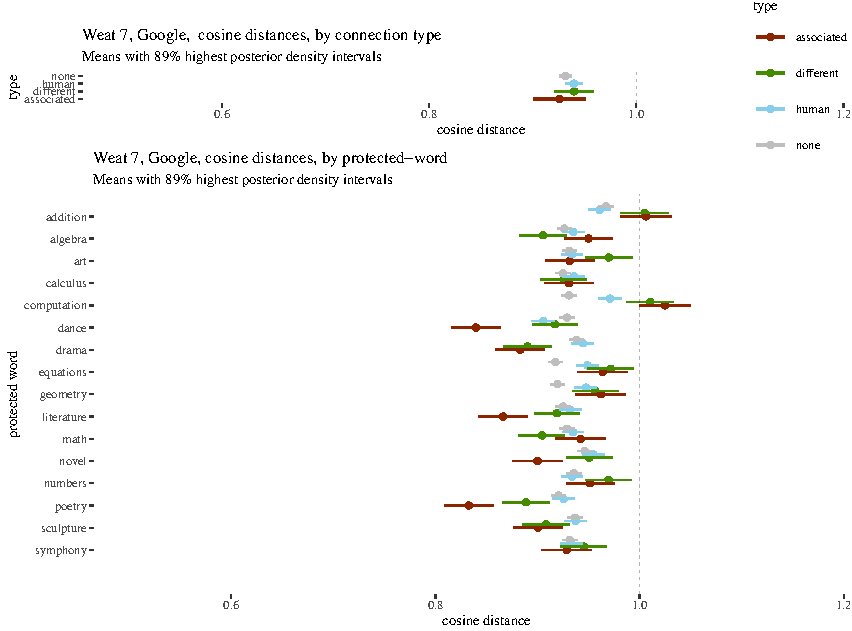
\includegraphics[width=1.1\linewidth]{paperDraft4_files/figure-latex/unnamed-chunk-2-1} \end{center}
\caption{dsds}
\label{fig:weat7google}
\end{figure}

\hypertarget{discussion-and-summary}{%
\section{Discussion and summary}\label{discussion-and-summary}}

\hypertarget{appendix}{%
\section{APPENDIX}\label{appendix}}

\hypertarget{examples-of-weat-and-mac-calculations}{%
\subsection{Examples of WEAT and MAC
calculations}\label{examples-of-weat-and-mac-calculations}}

\hypertarget{word-lists}{%
\subsection*{Word lists}\label{word-lists}}
\addcontentsline{toc}{subsection}{Word lists}

\hypertarget{refs}{}
\begin{CSLReferences}{0}{0}
\leavevmode\hypertarget{ref-Bolukbasi2016man}{}%
\CSLLeftMargin{{[}1{]} }
\CSLRightInline{Tolga Bolukbasi, Kai-Wei Chang, James Y. Zou, Venkatesh
Saligrama, and Adam Kalai. 2016. Man is to computer programmer as woman
is to homemaker? Debiasing word embeddings. \emph{CoRR} abs/1607.06520,
(2016). Retrieved from \url{http://arxiv.org/abs/1607.06520}}

\leavevmode\hypertarget{ref-Caliskan2017semanticsBiases}{}%
\CSLLeftMargin{{[}2{]} }
\CSLRightInline{Aylin Caliskan, Joanna J. Bryson, and Arvind Narayanan.
2017. Semantics derived automatically from language corpora contain
human-like biases. \emph{Science} 356, 6334 (April 2017), 183--186.
DOI:https://doi.org/\href{https://doi.org/10.1126/science.aal4230}{10.1126/science.aal4230}}

\leavevmode\hypertarget{ref-Garg2018years}{}%
\CSLLeftMargin{{[}3{]} }
\CSLRightInline{Nikhil Garg, Londa Schiebinger, Dan Jurafsky, and James
Zou. 2018. Word embeddings quantify 100 years of gender and ethnic
stereotypes. \emph{Proceedings of the National Academy of Sciences} 115,
16 (April 2018), E3635--E3644.
DOI:https://doi.org/\href{https://doi.org/10.1073/pnas.1720347115}{10.1073/pnas.1720347115}}

\leavevmode\hypertarget{ref-Gonen2019lipstick}{}%
\CSLLeftMargin{{[}4{]} }
\CSLRightInline{Hila Gonen and Yoav Goldberg. 2019. Lipstick on a pig:
{D}ebiasing methods cover up systematic gender biases in word embeddings
but do not remove them. In \emph{Proceedings of the 2019 conference of
the north {A}merican chapter of the association for computational
linguistics: Human language technologies, volume 1 (long and short
papers)}, Association for Computational Linguistics, Minneapolis,
Minnesota, 609--614.
DOI:https://doi.org/\href{https://doi.org/10.18653/v1/N19-1061}{10.18653/v1/N19-1061}}

\leavevmode\hypertarget{ref-Lauscher2019multidimensional}{}%
\CSLLeftMargin{{[}5{]} }
\CSLRightInline{Anne Lauscher and Goran Glavas. 2019. Are we
consistently biased? Multidimensional analysis of biases in
distributional word vectors. \emph{CoRR} abs/1904.11783, (2019).
Retrieved from \url{http://arxiv.org/abs/1904.11783}}

\leavevmode\hypertarget{ref-Manzini2019blackToCriminal}{}%
\CSLLeftMargin{{[}6{]} }
\CSLRightInline{Thomas Manzini, Yao Chong Lim, Yulia Tsvetkov, and Alan
W Black. 2019. Black is to criminal as caucasian is to police: Detecting
and removing multiclass bias in word embeddings. Retrieved from
\url{http://arxiv.org/abs/1904.04047}}

\leavevmode\hypertarget{ref-Nissim2020fair}{}%
\CSLLeftMargin{{[}7{]} }
\CSLRightInline{Malvina Nissim, Rik van Noord, and Rob van der Goot.
2020. Fair is better than sensational: Man is to doctor as woman is to
doctor. \emph{Computational Linguistics} 46, 2 (June 2020), 487--497.
DOI:https://doi.org/\href{https://doi.org/10.1162/coli_a_00379}{10.1162/coli\_a\_00379}}

\leavevmode\hypertarget{ref-Nosek2002harvesting}{}%
\CSLLeftMargin{{[}8{]} }
\CSLRightInline{Brian A. Nosek, Mahzarin R. Banaji, and Anthony G.
Greenwald. 2002. Harvesting implicit group attitudes and beliefs from a
demonstration web site. \emph{Group Dynamics: Theory, Research, and
Practice} 6, 1 (2002), 101--115.
DOI:https://doi.org/\href{https://doi.org/10.1037/1089-2699.6.1.101}{10.1037/1089-2699.6.1.101}}

\end{CSLReferences}

\end{document}
